\section{Lower Atmospheric Signatures of a Solar Flare Associated with Seismicity}
use old report content + new content in presentation (inc full page plots but better/bigger axis labels)

%\begin{itemize}
%\end{itemize}


\subsection{Background} 
Expand and de-itemize background (background should not be covering ground already in previous sections)


Sunquakes represent the propagation of acoustic waves in the sub-photosphere, responding to an excitation of the photosphere during the impulsive phase of solar flares. The progenitors of sunquakes are thought to be either shocks, radiative backwarming, direct particle collision or sudden magnetic field reconfiguration. Each of these mechanisms relies on the transport of energy from the corona to the photosphere, and the physical conditions existing in the chromosphere such as magnetic configuration and density. To understand sunquakes and their relationship to solar flares, we need to understand how energy moves down through the solar atmosphere and the physical conditions that are present. 

The majority of the energy released by a flare is deposited in the lower solar atmosphere and manifests itself in the form of enhanced hard X-ray, UV and optical radiation. During the impulsive phase of a solar flare, energy in the form of energetic particles, shocks and MHD waves flow along newly formed coronal magnetic loops, down through the stratified solar atmosphere. As energy is deposited through the differing enviroments of each atmospheric layer associated emission is released. 

Hard X-ray (HXR) footpoints are observed due to the excitation of the chromosphere by energetic particle beams accelerated by the reconnecting magnetic field in the the corona during the flare \citep{1995ApJ...455..347A}. According to the standard flare model \citep{1964NASSP..50..451C, 1966Natur.211..695S, 1974SoPh...34..323H, 1976SoPh...50...85K} magnetic reconnection in the corona leads to energy being directed downward in the form of particles, radiation, MHD waves and conduction of heat, which in turn produces ultra-violet (UV) ribbons in the chromosphere. This means that HXR footpoints and UV ribbons observed in the chromosphere directly map to the reconfiguring magnetic fields during the flare. 

As energy moves down through the chromosphere toward the photosphere, emission becomes visible in the optical, termed white light flare (WLF). The processes governing WLF emission in the lower solar atmosphere are detailed by \cite{2007ASPC..368..417D} whereby two main mechanisms are highlighted; Balmer/Paschen continuum emission produced via hydrogen recombination in the lower chromosphere; and enhancement of photospheric continuum emission due to heating of the temperature minimum region. According to \cite{1989SoPh..124..303M}, Balmer/Paschen emission upward (i.e., directly detected) also has a downward component which leads to radiative backwarming of the photosphere. Therefore WLF generation mechanisms are not mutually exclusive and can be expoited as a signature of energy deposition through the lower atmosphere. 


Using data collected by spacecraft observing the Sun, energy released during solar flares can be tracked as it is deposited throughout the atmosphere. 

Energy deposition in the corona and upper chromosphere is marked by HXR footpoints and UV ribbons. The Ramaty High Energy Solar Spectroscopic Imager (RHESSI) observes solar emission ranging from X-rays to $\gamma$-rays produced by energetic particles and nuclear interactions. RHESSI was designed with the aim of understanding impulsive energy release, particle acceleration and transportation in the magnetohydrodynamic environment of the solar atmosphere. Using 25 - 50 keV and 50 - 100 keV intensity data collected by RHESSI, HXR footpoints can be tracked and analysed. Observing UV ribbons requires a different spacecraft. The Interface Region Spectroscopic Imager (IRIS) captures near-ultraviolet (NUV) and far-ultraviolet (FUV) emission and is designed to observe the chromosphere at various altitudes. Emission is collected by a slit-jaw imager (SJI) and a spectrometer (SG) simultaneously. The spectrograph is sensitive in both FUV and NUV passbands, which expose 3 CCDs to produce spectra in three UV bands, two FUV and one NUV. Table \ref{iris-sg} shows how each passband relates to emission processes occurring from the upper-chromosphere down to the upper-photosphere. 


\begin{tabular}{|c|c|}\label{iris-sg}
Band & Wavelength ($\AA) & Temperature ($\log{T}$) & Region of Atmosphere\\ 
FUV 1 & $1331.7 - 1358.4$ & $3.7 - 7.0$ & Upper to lower-chromosphere\\ 
FUV 2 & $1389.0 - 1407.0$ & $3.7 - 5.2$ & Upper to lower-chromosphere\\ 
NUV & $2782.7 - 2851.1$ & $3.7 - 4.2$ & Lower-chromosphere to upper-photosphere\\ 
\caption{The IRIS/SG is capable of observing three passbands, which relate to different plasma temperatures.}  
\end{tabular}

The slit-jaw images, are light collected from a reflective area surrounding the slit. The imager is capable of observing four wavelengths relating to emission at different altitudes as shown by table \ref{iris-sj}. 

\begin{tabular}{|c|c|}\label{iris-sj}
SJI Passband & Wavelength ($\AA) & FWHM (\AA) & Temperature ($\log{T}$) & Region of Atmosphere\\ 
C II 1 & $1330$ & $40$ & $3.7 - 7.0$ & Upper-chromosphere\\ 
Si IV 2 & $1400$ & $40$ & $3.7 - 5.2$ & Upper-chromosphere\\ 
Mg II h/k & $2796$ & $4$ & $3.7 - 4.2$ & Lower-chromosphere\\ 
Mg II wing & $2832$ & $4$ & $3.7 - 3.8$ & Upper-photosphere\\   
\caption{}
\end{tabular}

  

Signatures from energy deposition in the lowest regions of atmosphere are captured by Solar Dymanics Observatory's (SDO) Helioseismic Imager (HMI), which observes the photosphere. Able to observe optical continuum intensity (6173Å), Helioseismic and magnetic data SDO/HMI can provide valuable data concerning WLFs, sunquakes and magnetic field configuration. Optical continuum data can provide information about WLFs and radiative backwarming of photospheric material, which is a possible sunquake progenitor. Helioseismic data can be used to analyse the movement of material during a solar flare, such as downward flows which could indicate shocks propagating from higher altitudes or particle beams penetrating the atmosphere. The point of origin and wavefronts of a sunquake can also be detected using helioseismic data, which can be used to calculate acoustic power of the quake. Magnetic data from SDO/HMI shows local magnetic field direction, useful for determining the presence of impulsive changes in magnetic field capable of generating a sunquake.     







\subsection{Observations}
More detailed




\begin{figure}\label{sunquake-cartoon}
  \begin{center}
  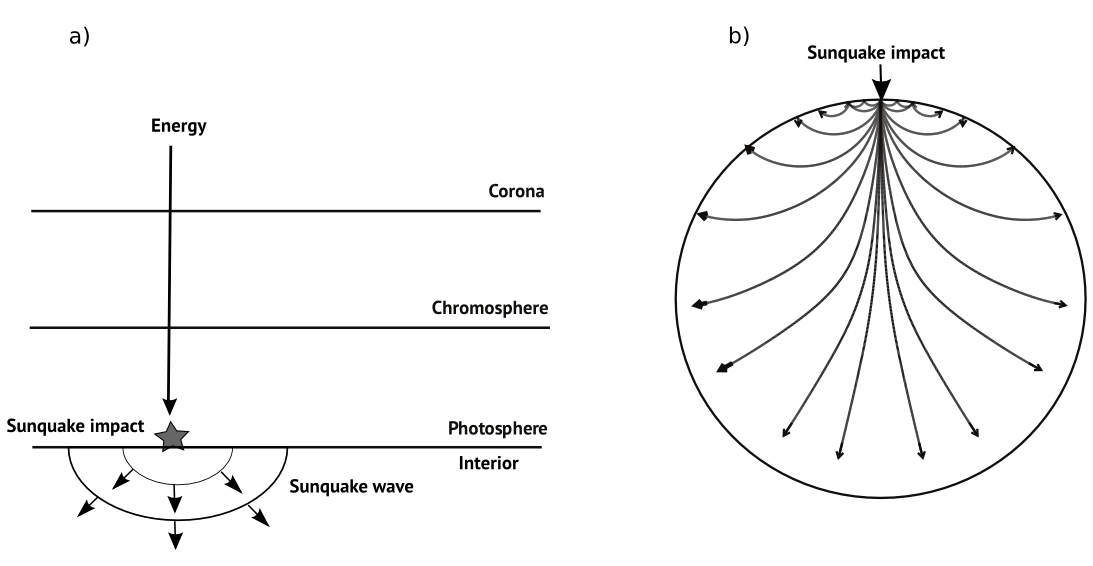
\includegraphics[width=0.40\textwidth]{sunquake-cartoon}
  \end{center}
  \caption{shows...}
\end{figure}




The X1 flare of the 29th of March 2014 at 17:46 UT in active region NOAA 12017, was observed by SDO, IRIS and RHESSI. HXR data from RHESSI, UV and Balmer emission from IRIS slit-jaw/spectrometer, and visible continuum from SDO HMI are observed during the flare.Balmer emission is taken from IRIS spectroscopic data (wavelength range of 2825.7 and 2825.8Å \citep{2014ApJ...794L..23H}. \\

\begin{figure}\label{saxcontours}
  \begin{center}
  \includegraphics[width=0.40\textwidth]{saxcontours}
  \end{center}
  \caption{From top to bottom shows IRIS Si IV slit-jaw, Mg II slit-jaw and SDO HMI continuum intensity maps.Contours show RHESSI HXR with $E = 25-50$ keV in white or black and HXR with $E = 50-100 keV$ in green, sunspot locations in yellow taken from HMI and 6mHz acoustic power in blue.}
\end{figure}





















\subsection{Analysis}
David Fanning Ladder plots. Analysis section should include more about techniques used to process the data.

\begin{figure}\label{sunquake-cartoon}
  \begin{center}
  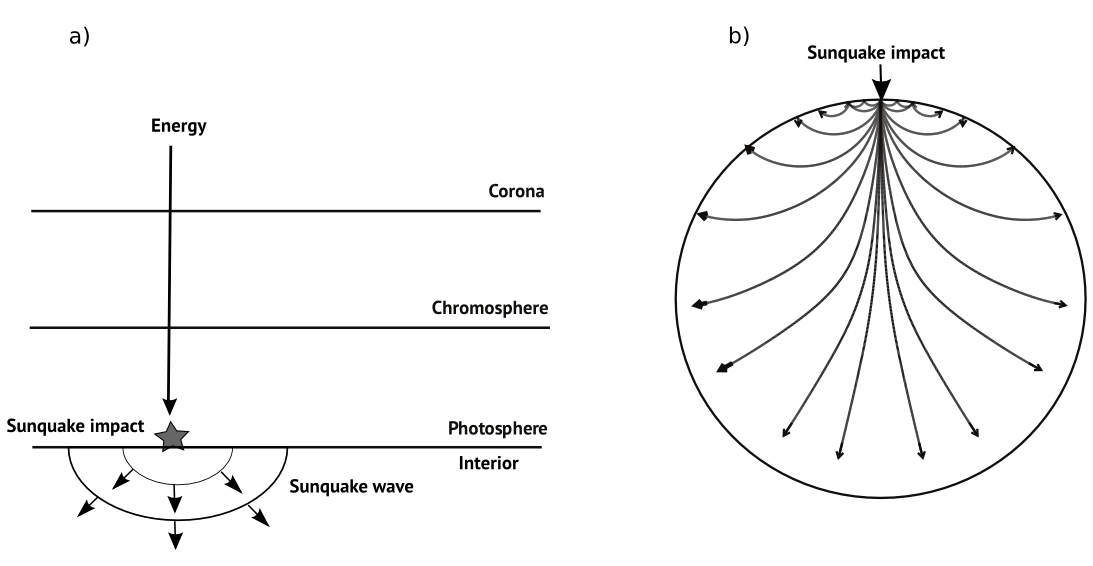
\includegraphics[width=0.40\textwidth]{sunquake-cartoon}
  \end{center}
  \caption{shows...}
\end{figure}


\subsection{Discussion}





\subsection{Future Work}



%%%%%%%%%%%%%%%%%%%%%%%%%%%%%%%%%%%%%%%%%%%%%%%%%%%%%%%%%%%%%%%%%%555
%old report content

\section{Project: Lower Atmospheric Signatures of Solar Flares Associated with Seismicity.}\label{PRJ}
%\begin{abstract}
%Sunquakes represent the propagation of acoustic waves in the sub-photosphere, responding to an excitation of the photosphere during the impulsive phase of solar flares. The progenitors of sunquakes are thought to be either shocks, radiative backwarming, direct particle collision or sudden magnetic field reconfiguration. Each of these mechanisms relies on the transport of energy from the corona to the photosphere, and the physical conditions existing in the chromosphere such as magnetic configuration and density. To understand sunquakes and their relationship to solar flares, we need to understand how energy moves down through the solar atmosphere and the physical conditions that are present. An X1 solar flare with associated sunquake was observed in active region NOAA 12017 on the 29th of March 2014 at 17:46 UTC, by multiple spacecraft, including SDO (HMI), IRIS and RHESSI. Lightcurves of the flare emission from the photosphere, chromosphere and transition region are analysed providing information about the deposition of energy at different altitudes in the solar atmosphere. Hard X-ray footpoints of coronal loops are shown to align well with an area associated with maximum acoustic power. Balmer continuum emission aligned with maximum acoustic power is shown to increase during the flare, indicating the existence of hydrogen recombination continua in the chromosphere possibly leading to radiative backwarming of the photosphere. 
%\end{abstract}

\subsection{Background}
Hard X-ray (HXR) footpoints (1) and UV ribbons (2) observed in the chromosphere directly map to the reconfiguring magnetic fields during the flare: 
1. HXR footpoints are observed due to the excitation of the lower atmosphere by electron particle beams accelerated by the reconnecting magnetic field in the the corona during the flare \citep{1995ApJ...455..347A}.
2.According to the standard flare model \citep{1964NASSP..50..451C, 1966Natur.211..695S, 1974SoPh...34..323H, 1976SoPh...50...85K} magnetic reconnection in the corona leads to energy being directed downward in the form of particles, radiation, MHD waves and conduction of heat, which in turn produces chromospheric ribbons.\\

The majority of the energy released by a flare is deposited in the lower solar atmosphere and manifests itself in the form of enhanced hard X-ray, UV and optical radiation. The production of a sunquake requires a fraction of less than 10-3 of the energy budget available during the flare \citep{2005ApJ...630.1168D}. \\


Optical emission in the lower atmosphere during a flare can occur via two mechanisms \citep{2007ASPC..368..417D}. 
1. Continuum emission from the photosphere is enhanced by heating of the temperature minimum region.
2. Balmer/Paschen continuum emission produced via hydrogen recombination in the chromosphere \\

Balmer/Paschen emission upward (i.e., directly detected) also has a downward component which leads to radiative backwarming of the photosphere \citep{1989SoPh..124..303M}. \\

Sunquakes occur as a result of solar flares depositing energy into the photosphere, stimulating the production of acoustic waves which propagate into the sub-photosphere. These acoustic transients travel into the interior of the sun until they refract back to the surface and are observed as concentric ripples in Dopplergrams \citep{2014arXiv1402.1249K}. \\

The method in which solar flares trigger sunquakes is unknown, although the following mechanisms are thought to be possible progenitors: shocks, radiative backwarming, direct particle collision and sudden magnetic field reconfiguration 



\subsection{Observations}
The X1 flare of the 29th of March 2014 at 17:46 UT in active region NOAA 12017, was observed by SDO, IRIS and RHESSI. HXR data from RHESSI, UV and Balmer emission from IRIS slit-jaw/spectrometer, and visible continuum from SDO HMI are observed during the flare.Balmer emission is taken from IRIS spectroscopic data (wavelength range of 2825.7 and 2825.8Å \citep{2014ApJ...794L..23H}. \\

\begin{figure}\label{saxcontours}
  \begin{center}
  \includegraphics[width=0.40\textwidth]{saxcontours}
  \end{center}
  \caption{From top to bottom shows IRIS Si IV slit-jaw, Mg II slit-jaw and SDO HMI continuum intensity maps.Contours show RHESSI HXR with $E = 25-50$ keV in white or black and HXR with $E = 50-100 keV$ in green, sunspot locations in yellow taken from HMI and 6mHz acoustic power in blue.}
\end{figure}



\subsection{Analysis}
SDO HMI data is subjected to a running difference filter to isolate locations that appear to flare in white light . These enhanced pixels are identified by using a combination of visual inspection and thresholding to eliminate false positives being triggered by noise of similar intensities.Lightcurves are created from SDO HMI continuum processed data. IRIS slit jaw images of Si IV and Mg II are aligned with HMI and lightcurves are created \ref{lcseries} for pixels at the quake and ribbon locations. Lightcurves are created from IRIS spectroscopic data at slit positions aligned with quake and ribbon locations, over a wavelength range within the Balmer continuum. IRIS spectroscopic data are analysed at sunquake, ribbon and non-flaring positions. An egression map of acoustic power is produced  at 6mHz, revealing the position of the sunquake. HXR data from RHESSI and acoustic power data are overlaid on HMI and IRIS slit jaw maps.\\

\begin{figure}\label{lcseries}
  \begin{center} 
\includegraphics[width=0.48\textwidth]{lcseries}
  \end{center}
  \caption{Left panel shows data over the quake location, right panel shows data over the ribbon location. From top to bottom, plots show lightcurves from IRIS Si IV, Mg II and Balmer wavelengths, with the bottom panel showing the lightcurve from SDO HMI. }
\end{figure}

\begin{figure}\label{spectra}
  \begin{center}
  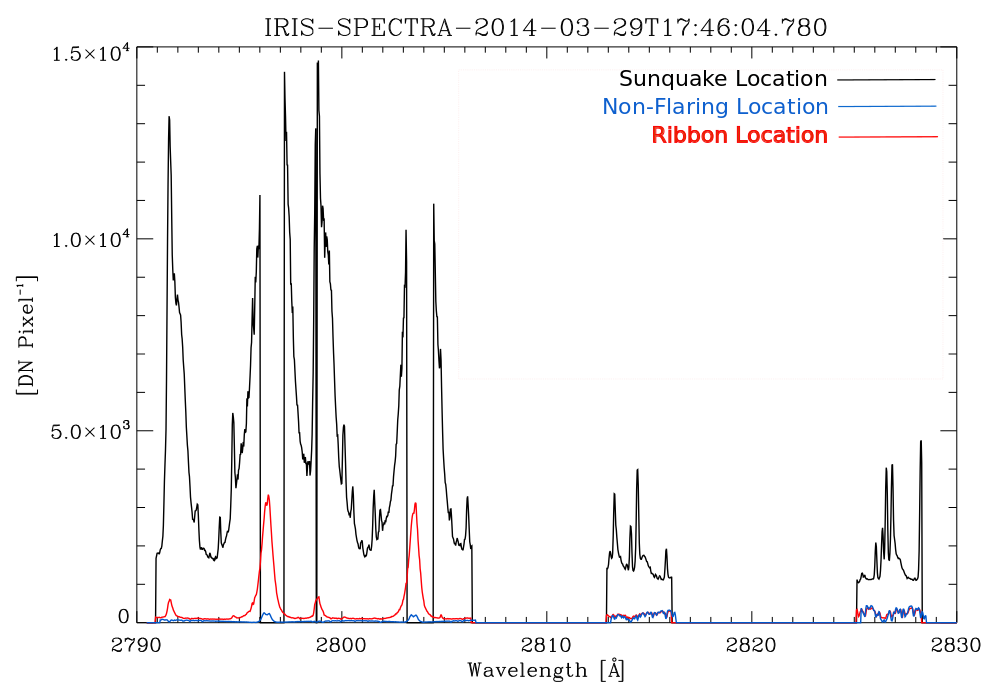
\includegraphics[width=0.58\textwidth]{spectra}
  \end{center}
  \caption{IRIS spectroscopic data ranging in wavelength 2796 - 2830Å with a smaller plot showing a zoom of the region containing the Mg II triplet lines. Black is the spectrum at the quake location (y = 435), red is the spectrum at a point along the ribbon (y = 489) and blue is the spectrum of a non-flaring region (y = 20). Square trough like features represent saturation of the CCD.}
\end{figure}
 

\subsection{First Results and Discussion}
The location of maximum acoustic power, RHESSI HXR, IRIS and SDO intensity correlate both spatially and temporally \ref{saxcontours}, showing that energy input into the upper chromosphere somehow propagates down to the photosphere. Intensity lightcurves \ref{lcseries} from SDO and IRIS seem to suggest a similar representation of the movement of energy through the chromosphere to lower altitudes, since their impulsive appearance and peak intensity occur within a minute of each 
other throughout the different regions. Intensity contrast values shown in \ref{lcseries} give an idea of how much energy is being deposited in each part of the atmosphere but energy calculations are needed. A highly impulsive Balmer continuum \ref{lcseries}, at sunquake and ribbon locations, shows that there is likely to be some radiative backwarming involved in passing energy to the photosphere. Spectroscopic data shown in \ref{spectra} show the sunquake emission to be an order of magnitude greater in amplitude than in the ribbon. The spectrum taken from a non-flaring region is around three orders of magnitude smaller than the sunquake location. Lines over the sunquake location are strongly broadened when compared to spectra elsewhere \ref{spectra}. Ribbon and sunquake spectra appear to be slightly redshifted in comparison to the non-flaring region.\\


\subsection{Future Work}
Calculate energy associated with emission captured by HMI to compare with the acoustic power of the sunquake. Calculate energy associated with emission captured by IRIS slit jaw and spectrometer in order to estimate energy deposition in the atmosphere. Calculate energy associated with Balmer emission to assess likely energy contribution of radiative backwarming. Calculate non-thermal electron power via HXR spectra to estimate the initial energy of the electron beam accelerated by the corona. A more detailed analysis of IRIS spectroscopic data to estimate velocity, density and temperature of chromospheric material. Analysis of triplet lines in the wings of Mg II h \& k will be used to determine heating of the lower chromosphere. Compare spectroscopic data taken by EIS with that of IRIS. Magnetogram: Look at HMI/SOT data to analyse the configuration of the magnetic field.\\
